%% Section 6: Primary Results
%% STATUS: STUB — table shells and figure placeholders present.
%% See artifacts/revision2/SIGMETRICS_OUTLINE.md §6 for planned content (~2.5 pages).

\section{Primary Results}
\label{sec:results}

\subsection{Primary Endpoint (H4): FP vs.\ Random at $r=1.25$}
% source: artifacts/revision2/challenge_analysis.json
%   FP_vs_Random r=1.25:
%     median_delta_lo = 6.706290619727605 -> +6.71 pp
%     bootstrap95_delta_lo = [3.9196535626004456, 8.72485557161271] -> [+3.92,+8.72]
%     n_definitely_A = 22, n_indistinguishable = 1, n_definitely_B = 2
%     interpretation.H4_primary_success.pass = true

\subsection{Node-Specificity Test: FP vs.\ Within-Cabinet Placebo}
% source: artifacts/revision2/challenge_analysis.json
%   FP_vs_WithinCabPlacebo r=1.25:
%     median_delta_lo = 3.537760317644416 -> +3.54 pp
%     bootstrap95_delta_lo = [0.5580646330144061, 4.435295391457885] -> [+0.56,+4.44]
%     n_definitely_A = 20, n_indistinguishable = 5, n_definitely_B = 0

\subsection{Factorial Comparison Table}

\begin{table}[t]
\caption{Factorial comparison results at the pre-specified $r=1.25$ choice ratio.
$\delta_{\mathrm{lo}} = C_{\mathrm{lower}}(A) - C_{\mathrm{upper}}(B)$ is the
conservative bracket separation. A: definitely A better; I: indistinguishable;
B: definitely B better. All values from 25 held-out scenarios (sc30--sc54).}
\label{tab:factorial}
\centering
\begin{tabular}{lrrr}
\toprule
Comparison & A\,/\,I\,/\,B & Median $\delta_{\mathrm{lo}}$ & Bootstrap 95\%~CI \\
\midrule
\textbf{FP vs.\ Random} (primary)        & \textbf{22\,/\,1\,/\,2}  & $+6.71$ pp & $[{+}3.92, {+}8.72]$ \\
\textbf{FP vs.\ WithinCabPlacebo}        & \textbf{20\,/\,5\,/\,0}  & $+3.54$ pp & $[{+}0.56, {+}4.44]$ \\
FP vs.\ GlobalPlacebo                    & 22\,/\,1\,/\,2            & $+4.55$ pp & $[{+}2.95, {+}7.82]$ \\
FPSpread vs.\ RandomSpread               & 20\,/\,5\,/\,0            & $+2.15$ pp & $[{+}0.52, {+}4.25]$ \\
RandomSpread vs.\ Random                 & 8\,/\,14\,/\,3            & $+0.00$ pp & $[{-}0.26, {+}0.03]$ \\
FPSpread vs.\ FP                         & 4\,/\,3\,/\,18            & $-2.64$ pp & $[{-}4.49, {-}2.00]$ \\
FP vs.\ PositionTemplate                 & 16\,/\,5\,/\,4            & $+0.74$ pp & $[{-}0.82, {+}1.50]$ \\
FPSpread vs.\ PositionTemplate           & 6\,/\,11\,/\,8            & $-1.16$ pp & $[{-}2.29, {-}0.25]$ \\
\bottomrule
\end{tabular}
% source: artifacts/revision2/challenge_analysis.json (all rows verified in
%         FINAL_NUMERICAL_CLAIM_AUDIT.md V8-V24)
% Floor/left-censored note for FP_vs_Random:
%   full_random: 9 base-infeasible (left_boundary, [0,0]) + 3 floor-at-zero (exact_bracket, C_lower=0) = 12 total C_lower=0
%   full_fp: 0 base-infeasible, 0 floor
%   n_both_left_censored: 0 (FP never base-infeasible at r=1.25)
%   First binding constraint for random base-infeasible scenarios: B=8, S=1
% RandomSpread_vs_Random n_both_left_censored: 6 (both policies base-infeasible in same 6 scenarios)
% These scenarios are not "ties at zero"; they are base-infeasible and excluded from bracket-width summaries.
% source: per-scenario crossing data in artifacts/revision2/results/gate_f_sc*_all_r2challenge.json
\end{table}

\subsection{Factorial Pattern Interpretation}
% TODO: Discuss interpretation — global placebo, spreading decomposition,
% negative control, position template non-separation.

% Figure 3: Primary challenge forest plot
\begin{figure}[t]
\centering
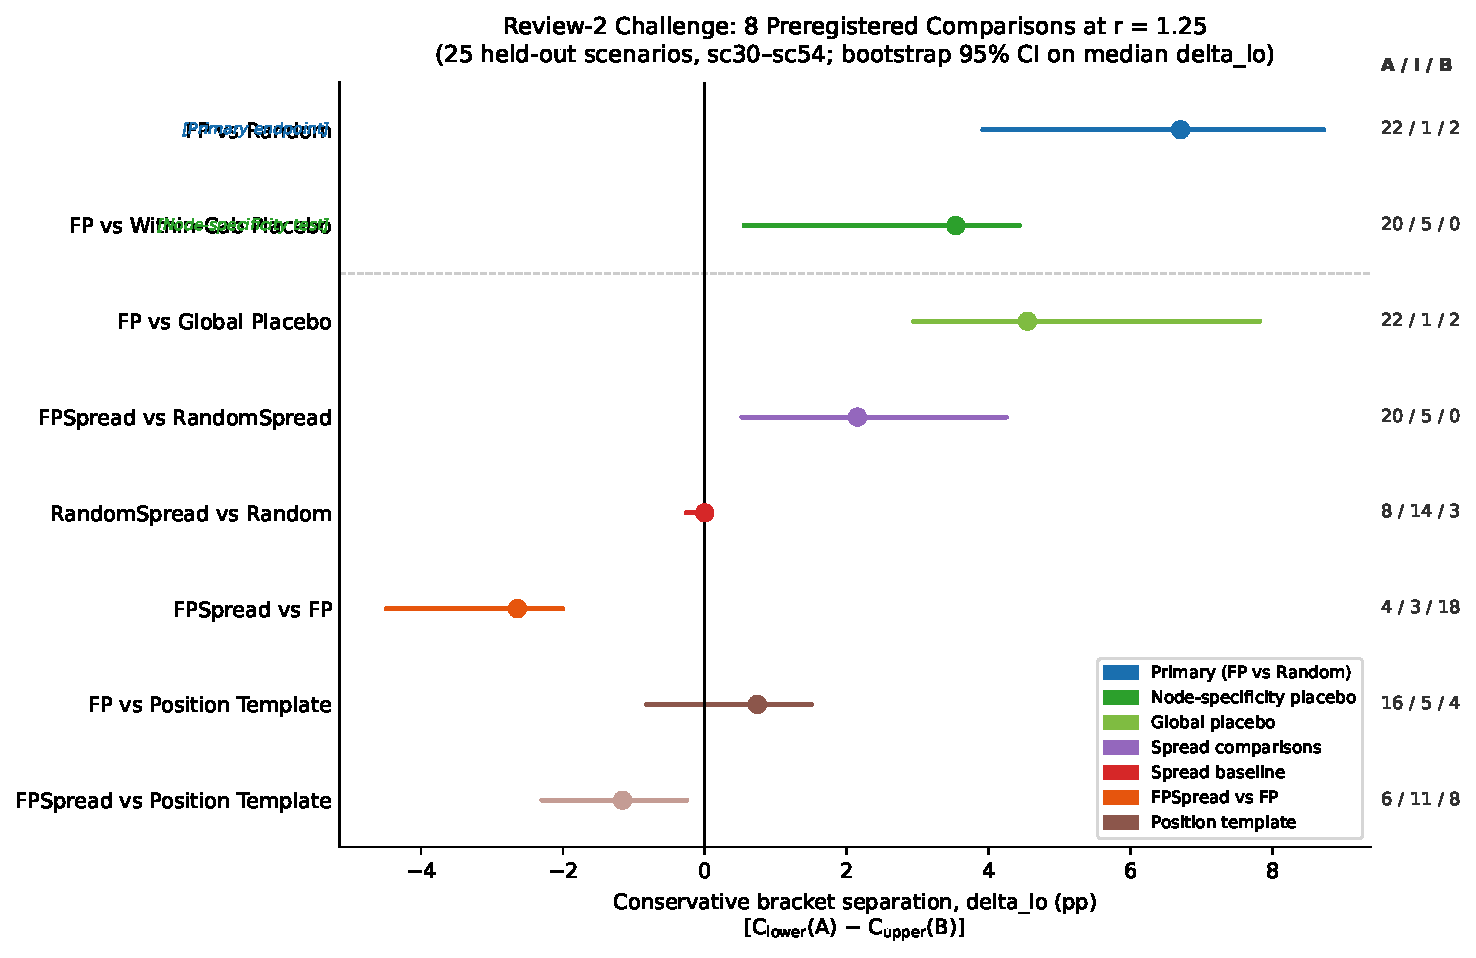
\includegraphics[width=0.85\textwidth]{fig_r2_factorial_r125}
% source: artifacts/revision2/figures/fig_r2_factorial_r125.pdf (300 dpi)
% generation: artifacts/revision2/figures/fig_r2_main.py
\caption{Forest plot of 8 pre-specified comparisons at $r=1.25$.
Each row shows the median conservative bracket separation $\delta_{\mathrm{lo}}$
with bootstrap 95\%~CI. A/I/B counts (definitely-A / indistinguishable /
definitely-B) shown at right. All 25 held-out scenarios (sc30--sc54).}
\label{fig:factorial}
\end{figure}

\subsection{Pre-specified Secondary Finding: FPSpread Crossover}

% Figure 4: FPSpread crossover
\begin{figure}[t]
\centering
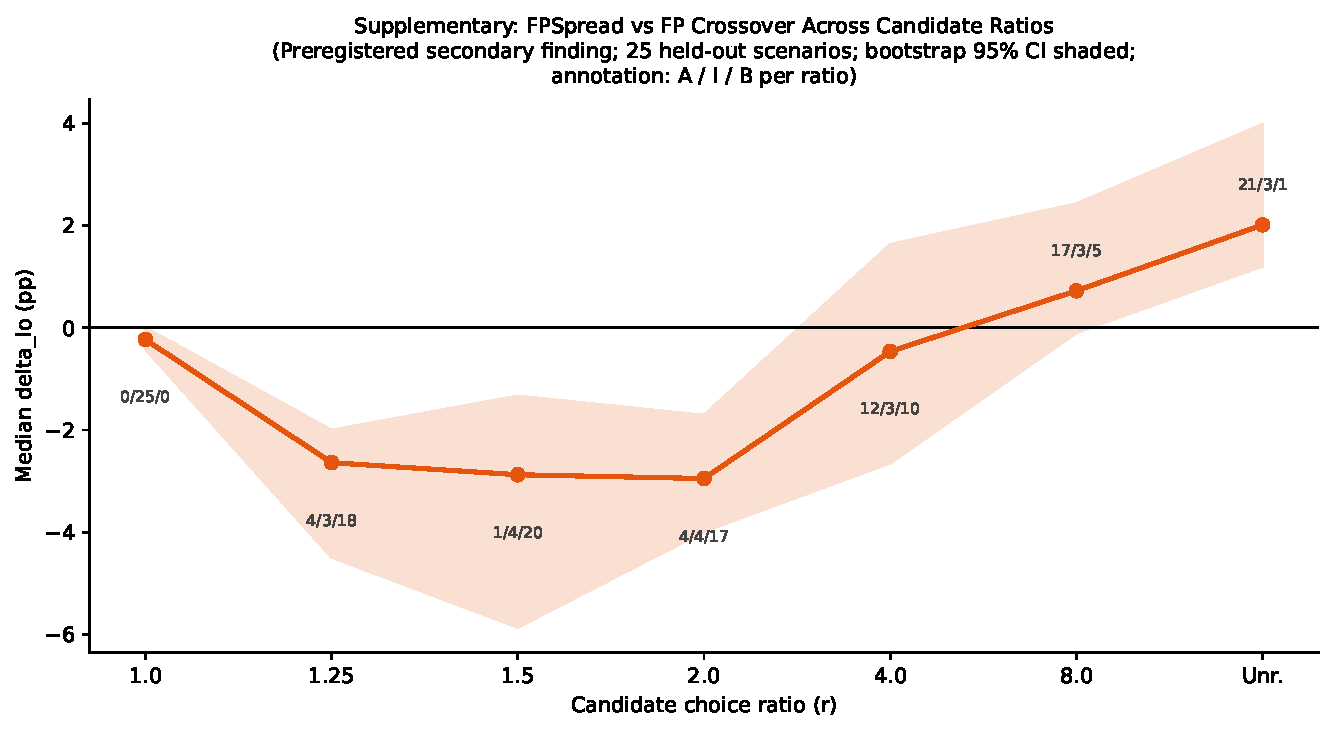
\includegraphics[width=0.75\textwidth]{fig_r2_fpspread_crossover}
% source: artifacts/revision2/figures/fig_r2_fpspread_crossover.pdf (300 dpi)
% generation: artifacts/revision2/figures/fig_r2_main.py
\caption{FPSpread vs.\ FP across candidate choice ratios (pre-specified secondary finding). FPSpread underperforms FP at constrained ratios ($r=1.25$--$2.0$) and
outperforms at large choice sets ($r\geq8.0$, unrestricted). Values from
challenge\_analysis.json; shaded region is bootstrap 95\%~CI.}
\label{fig:crossover}
\end{figure}

% source for crossover table: artifacts/revision2/challenge_analysis.json
%   FPSpread_vs_FP r=1.25: -2.640 pp  (4/3/18)
%   FPSpread_vs_FP r=1.5:  -2.876 pp  (1/4/20)
%   FPSpread_vs_FP r=2.0:  -2.951 pp  (4/4/17)
%   FPSpread_vs_FP r=4.0:  -0.464 pp  (12/3/10)
%   FPSpread_vs_FP r=8.0:  +0.722 pp  (17/3/5)
%   FPSpread_vs_FP unr:    +2.012 pp  (21/3/1)

\subsection{Negative Control}
% All 8 comparisons at r=1.0: 0 / 25 / 0.
% source: artifacts/revision2/challenge_analysis.json
%   H5_r1_negative_control.all_indistinguishable = true
